\section{Usage Examples}
\label{sec-usage}

% 10 Dec 2012 : GWA : TODO : Numbers.

This section presents five \PhoneLab{} usage examples. Each vignette begins by
highlighting an interesting or important aspect of the usage data we have
collected. Our goal, however, is not to conduct an exhaustive analysis.
Instead, each example continues by discussing how the presented results would
guide the design of future \PhoneLab{} experiments.

\subsection{Overall Battery Usage}
\label{subsec-batteryoverview}

\begin{figure*}[t]
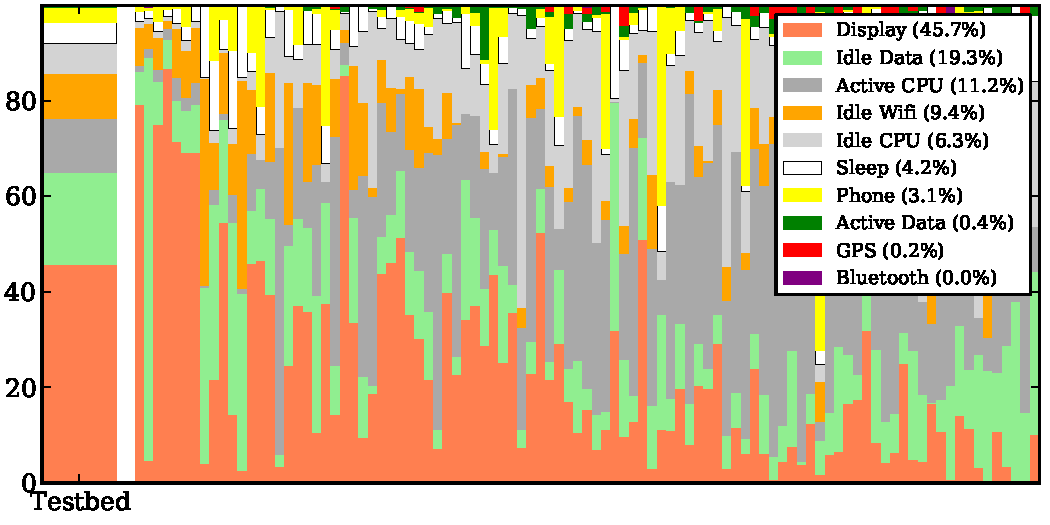
\includegraphics[width=\textwidth]{./figures/power/breakdown/graph.pdf}
\caption{\textbf{Power usage by component.} The large bar at left shows an
aggregated breakdown for the entire testbed. The participant bars are scaled
against the participant with the most energy usage.}
\label{figure-batteryoverview}
\end{figure*}

Smartphones are constrained by power, and a large amount of research on
smartphone systems is motivated by energy
conservation~\cite{shye:micro:2009,banerjee:ubicomp:2007,ace-mobisys12}. While
power is a definite concern, evaluating the potential impact of energy saving
approaches requires an accurate breakdown of where energy is used by real
phones. Only then can we be sure we are addressing actual energy bottlenecks and
use Amdahl's law to put relative energy savings into context.

\subsubsection{Energy Breakdown}

A component-by-component breakdown for the entire testbed and per-participant
is shown in Figure~\ref{figure-batteryoverview}. Our results are similar to
those reported by other studies, and indicate that mobile data, the screen,
and CPU usage are the main sources of smartphone power consumption. The
per-participant bars also show a great deal of variation, with differences in
both the amount and the breakdown of energy consumed by each participant.

One supposedly power-hungry component that has less of an impact than we had
expected is the GPS. This is particularly surprising given the large amount
of location-monitoring work motivated by GPS power consumption. One of
several factors may be at work. First, the Android platform estimates the GPS
chipset current consumption at 50~mA. This number is used by the standard
``Fuel Guage'' battery monitor and by our calculations. However, it is lower
than the data sheet for the part~\cite{FIXME} and may represent a best-case
average. However, increasing the GPS current by a factor of four does not
significant increase its contribution: from \XXXnote{GWA} to \XXXnote{GWA}.

Other hypothesis are that Android network location is providing location with
sufficient accuracy for many applications, eliminating the need for GPS. Or,
participants and applications may simply be conscious of GPS power
consumption and taking active steps to control it.

\subsubsection{Future Experiments}

While previous smaller studies on earlier Android
models~\cite{shye:micro:2009} have presented similar taxonomies, the process
of identifying energy bottlenecks must be repeated regularly as hardware and
user behavior changes. \PhoneLab{} provides an ideal environment for
repeating energy usage experiments. Access to a stable set of participants
allows us to identify changes due to participant behavior, as participants
develop an awareness of the power consumption properties of their phones and
how to control them. And as we bring new hardware onto the testbed, we can
repeat power usage experiments to determine differences between smartphone
hardware generations.
